\documentclass[conference, 10pt]{IEEEtran}
\usepackage{hyperref}
\usepackage{url}
\usepackage{latexsym}
\usepackage{graphicx}
\usepackage{amsmath}
\usepackage{amsthm}
\usepackage{amssymb}
\usepackage{amsfonts}
\usepackage{epsfig}
\usepackage{cite}
\usepackage{calc}
\usepackage{color}
\usepackage{subfigure}
\usepackage{algorithm}
\usepackage{algpseudocode}
%\usepackage{enumitem}
%\usepackage{lipsum}


\DeclareGraphicsExtensions{.jpg, .eps}
%\DeclareGraphicsRule{.jpg}{eps}{.jpg.bb}{`jpeg2ps -h -r 600 #1} 

\newtheorem{thm}{Theorem}
\newtheorem{cor}{Corollary}
\newtheorem{lem}{Lemma}
\newtheorem{prop}{Proposition}
\newtheorem{defn}{Definition}
\newtheorem{ex}{Example}
\newtheorem{remark}{Remark}

%\newcommand{\alglabel}[1]{\newcounter{#1}\setcounter{#1}{\value{ALC@line}}}
%\newcommand{\algref}[1]{\arabic{#1}}
\newcommand{\abs}[1]{\lvert #1 \rvert}
\newcommand{\flr}[1]{\lfloor #1 \rfloor}
\newcommand{\cel}[1]{\lceil #1 \rceil}
\newcommand{\mc}[1]{{\mathcal{#1}}}
\newcommand{\card}[1]{\abs{#1}}
\newcommand{\norm}[1]{{\|{#1}\|}}
\newcommand{\normsq}[1]{{\|{#1}\|}^2}
\newcommand{\ind}[1]{{\mathbb I}_{\{#1\}}}
\newcommand{\wedef}{\stackrel{\triangle}{=}}
\newcommand{\nth}[1]{{#1}^{\text{th}}}
\newcommand{\smfrac}[2]{{\textstyle{\frac{#1}{#2}}}}
\newcommand{\mybox}{\raisebox{3pt}{$\fbox{}$}}
\newcommand{\comm}[1]{{\bf COMMENT:} #1}
\newcommand{\mU}{{\mathcal{U}}}
\newcommand{\tr}{{\tilde{r}}}
\newcommand{\tX}{{\tilde{X}}}
\newcommand{\tL}{{\tilde{L}}}
\newcommand{\mM}{{\mathcal{M}}}
\newcommand{\mP}{{\mathcal{P}}}
\newcommand{\mI}{{\mathcal{I}}}
\newcommand{\mJ}{{\mathcal{J}}}
\newcommand{\mL}{{\mathcal{L}}}
\newcommand{\mO}{{\mathcal{O}}}
\newcommand{\bp}{{\mathbf{p}}}
\newcommand{\bb}{{\mathbf{b}}}
\newcommand{\bg}{{\mathbf{g}}}
\newcommand{\bz}{{\mathbf{z}}}
\newcommand{\bm}{{\mathbf{m}}}
\newcommand{\bK}{{\mathbf{K}}}
\newcommand{\mD}{{\mathcal{D}}}
\newcommand{\bA}{{\mathbf{A}}}
\newcommand{\ba}{{\mathbf{a}}}
\newcommand{\Ex}{{\mathbb{E}}}
\newcommand{\bPi}{{\boldsymbol{\Pi}}}



%\newcommand{\bpf}{\begin{proof}}
%\newcommand{\epf}{\end{proof}}
%\newcommand{\bdefn}{\begin{defn}}
%\newcommand{\edefn}{\end{defn}}
%\newcommand{\bprf}{{\em Proof: }}
%\newcommand{\bproof}{{\em Proof of }}
%\newcommand{\eproof}{\hfill $\Box$}
%\newcommand{\fix}{\marginpar{FIX}}
%\newcommand{\new}{\marginpar{NEW}}

%%%%%%%%%%%%%%%%%%%%%%%%%%%%%%%%%%%%%%%%%%%%%%%%%%%%%%%%%%%%%%%%%%%%%%%%%%%%%%%%%%%
\iffalse


- Motivation and Localization Problem

- Our approach

- Machine Learning Problem Statement

- Algorithm

- Extension to observation modeling

- Results

\fi

\title{Localization of 5G Measurement Records}
% author names and affiliations
\author{Paper Id: xxxx}
%\author{\IEEEauthorblockN{XXX, XXX}
%\IEEEauthorblockA{Nokia \\
%Murray Hill, NJ, USA \\
%\emph{\{xxx, xxx\}@nokia.com}}
%}



\begin{document}
\maketitle

%\setlist[itemize]{leftmargin=*}

\begin{abstract}

% As cellular networks like 4G~LTE networks get more and more sophisticated, mobiles
% also measure and send enormous amount of mobile measurement data (in
% TBs/week/metropoliton) during every call and session. The mobile measurement records
% are saved in data center for further analysis and mining, however, these measurement
% records are not geo-tagged because the measurement procedures are implemented in
% mobile LTE stack. Geo-tagging (or localizing) the stored measurement record is a
% fundamental building block towards network analytics and troubleshooting since the
% measurement records contain  rich information on call quality, latency, throughput,
% signal quality, error codes etc. In this work, our goal is to localize these mobile
% measurement records. Precisely, we answer the following question: {\em what was the
% location of the mobile when it sent a given measurement record?} We design and
% implement novel machine learning based algorithms to infer whether a mobile was
% outdoor and if so, it infers the latitude-longitude associated with the measurement
% record. The key technical challenge comes from the fact that measurement records do
% not contain sufficient information required for triangulation or RF fingerprinting
% based techniques to work by themselves. Experiments performed with real data sets
% from an operational 4G network in a major metropolitan show that, the median accuracy
% of our proposed solution is around 20~m for outdoor mobiles and outdoor
% classification accuracy is more than $98\%$.

\end{abstract}

%\let\labelindent\relax

\section{Introduction}


%Importance of measurements

Fuled with the emerging cloud technologies (cloud computing, cloud storage, etc), software defined network (SDN) together with 
network functions virtualization (NFV) is transforming the techonology, and business models in telcommunication industry.
Several open source platforms (ONAP, XRAN, etc) have emerged to provide a platform to collect data and share technogies among different 
vendors and operators. As the wireless network is now evolving into 5G, tremendous data will be shared in these open source platform and thus create 
a lot of opportunity to provide better service using these data. These data can include a wide variety of measurements, such as the service throughput of the mobile 
device, the serving cell, the signal strength, etc. In ~\cite{Pantelis2016Localization}, a novel localization algorithm has been proposed to estimate 
the location when measurement reports are made in LTE systems. The paper shows that the medium accuracy of 20m can be achieved for outdoor mobibles. 
When celluar network evloves from 4G LTE to 5G, a lot of changes have been made to support lower latency and higher throughput. The most profound advanced technology adopted in 5G
network is the utilization of the massive multiple input multiple output (MIMO) antennas. With the usage of massive MIMO, the mobile will report beam related metric to the base station. 
In this paper, we propose a new localization algorithm to estiamte the location of the measruement report utilizing the new reported metric introduced in 5G network.
 

%Our goal - loc and class
As the open source platform is a new platform under development, it provivdes an opportunity to request different measurement 
metric. 
The goal of this work is two folds: 1). identify the measuremnets unique to 5G network for localization.
2). to estimate the latitude-longitude of the mobile when the measurement record was
generated for 5G network. 
%Our approach

In this paper, we combine the localization principles based on RF 
fingerprinting and probablitistic path-tracking used for robot localization, which is similar to ~\cite{Pantelis2016Localization}. However, different from ~\cite{Pantelis2016Localization}, the unique property of 5G network, such as the beamrelated 
information is used in this paper. The focus of this paper is on estimating location for outdoor mobiles. 
At a high level, our approach has two steps for
localizing measurement records from outdoor mobiles:

\begin{enumerate}
\item Instead of viewing each LUMD record in isolation, for each mobile, we {\em stitch}
together LUMD records from that mobile over a ``session
duration"  and model it as a suitable Markovian time series. The problem now
reduces to identifying locations (states) of the entire path of
the mobile.

\item The above solution method assumes that the probabilities characterizing the
underlying Markovian structure can be learned. This is done by performing supervised learning using the unique property of 5G networks.
The training data for supervised learning may come from
drive test carried out by network providers once 5G is deployed commein the field. However, given 5G network is not available in the field now, 
in this paper, we generate the drive training data and testing data from a 5G simulator.
	
\end{enumerate}

The details of the above two steps are provided in Section~\ref{sec:localalgo}.


Our main contribution in this paper is that we have proposed a new localization algorithm
appliable to 5G network. Based on our best knowledge, this is the first localization algorithm designed for 5G network. 


The rest of the paper is organized as follows. Section~\ref{sec:bg} provides some
background and introduces relevant terminologies. Section~\ref{sec:ps} presents
the problem setting and states the precise localization problem.
Section~\ref{sec:localalgo}
presents the main localization algorithm and Section~\ref{sec:extensionalgo} describes the extension of the joint localizationa and observation model estimation algorithm. 
We present experimental validation in Section~\ref{sec:eval} and finally we conclude in
Section~\ref{sec:concl}.

%Contributions



\section{Relevant 5G Terminologies}
\label{sec:bg}
NOTE: This section needs to be updated. Now, it is copied from previous paper, thus, it is about LTE.

Though our techniques could apply to any future cellular system, we use LTE
terminologies for convenience. The terminologies~\cite{ltebook} relevant for our purpose are
described below.

{\em UE (user equipment):} UE refers to the mobile end-device.

{\em Cell:} In LTE networks, a cell refers to coverage footprint of a base station
transmitter typically ensuring a cell coverage radius around 0.5~km-5~km.  In LTE
macro cells, each cell typically has a directional base-station transmitter with
$120^\circ$ sectorized antennas.

{\em gNodeB (gNB):} The eNB is the network element that interfaces with the UE and
hosts critical protocol layers like PHY, MAC, and Radio Link Control (RLC) etc. Each
eNB typically has 3~base station transmitters with $120^\circ$ antennas.

{\em Reference Signal Received Power (SSSRP):} In LTE networks, UEs make certain
measurements of received signal strength for each nearby cell transmitter. RSRP is
the total measured time-average received power at UE of all downlink reference
signals across the entire bandwidth from a {\em given cell transmitter}. RSRP is a
measure of the received signal strength of a cell transmitter at a UE.

{\em beam indices:} RSSI (Received Signal Strength Indicator) is the total measured
received power at the UE over the entire band of operation from {\em all cell
transmitters.} RSRQ of a given cell transmitter at a UE is RSSI scaled by average
RSRP (of that cell) per reference symbol.

We will need a figure to show the connection of 5G network to ONAP/xRAN, etc where the measured 
data is stored.

\begin{figure}[t]
\begin{center}
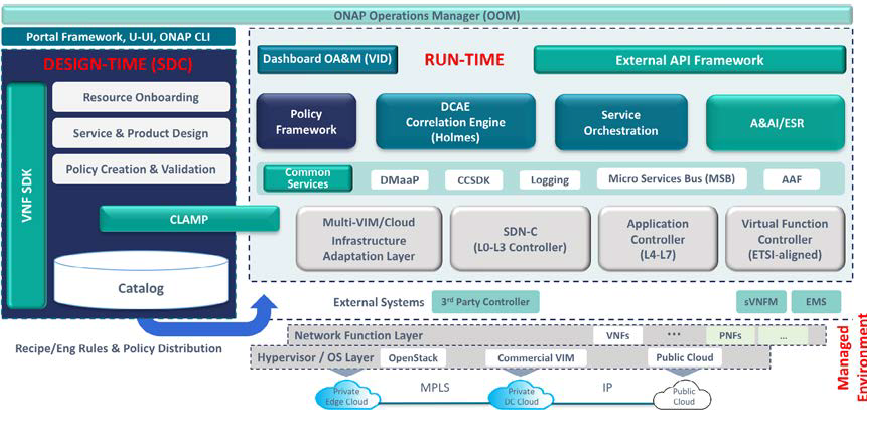
\includegraphics[height=3.5in,width=3.2in]{./ONAP-architecture.png}
\caption{\label{fig:lumd_arch}
{\small LUMD Data Collection.}}
\end{center}
\end{figure}



{\em Measurement data collection architecture:} The LUMD data collection architecture
is shown in Figure~\ref{fig:lumd_arch}. LUMD is collected at both the eNodeB and MME
(Mobility Management Entity). The MME serves as the coordinator of the LUMD data.
After LUMD collection is turned on at the eNodeB, it collects the records and sends
the data to the MME. MME aggregates and temporarily saves LUMD from multiple
eNodeBs and sends it periodically (typically in minutes time-scale) to the data
center where LUMD is saved and analyzed. Scalable storage of LUMD, which can easily
run into TB in a week per metropolitan, in the data center is an important design
problem and beyond the scope of this paper.


{\em Contents of LUMD:} LUMD record contains data related to signaling performance on
per UE, per bearer level for different procedures, user experience such as data
throughput and procedure duration, eNodeB internal UE related data such as MIMO
decision, SINR, buffer size, and normalized power headroom etc.  What information is
present depends on procedure/event that led to the measurement record. For our
purpose, we are interested in RF information contained in measurement records. These
are RSRP and RSRQ information. A LUMD record contains the following RF information:

\begin{itemize}

\item {\em RSRP:} Most LUMD contain RSRP of the serving cell that a UE is associated
with. In addition, only when LUMD is generated due to an A3 or A4 event as described
earlier in this section, it might also contain the RSRP of {\em one} neighboring
cell (typically the strongest one).

\item {\em beam indices:} LUMD also contains RSRQ of the serving cell. Note that once RSRP
and RSRQ are known, the corresponding RSSI can be uniquely computed since RSRQ is
defined as RSSI scaled by RSRP per reference symbol.

\end{itemize}

The important thing to note is that RSRP and RSRQ information is available from no
more than two cells in an LUMD record.


%mobile measurement data, system, pcmd, data center, period



\section{Problem Statement} 
\label{sec:ps}

Consider in an 5G network, mobiles travel along a road network represented by a graph $G_r=(V,E)$ where $V$
denotes graph nodes represented by a latitude-longitude tuple and $E$ denotes
valid direct path between two nodes.

There are two two types of data relevant to our discussion:

\begin{enumerate}

\item \textbf{Training data:} This is essentially geo-tagged data sent from
a set of locations in the road graph nodes $V$. Precisely, we are given $n$ locations
$\{x_i\}_{i=1}^n$ and for each location, up to four SSSRPs and beam indices of
the serving cell. Note that standard allows each UE to report up to four best beam indices and corresponding SSSRPs.
We denote by $\{B^{j}_{i,k}\}_{i=1}^n$, the jth best beam indices sent from training location $x_i$ with cell $k$ and $\{R^j_{i,k}\}_{i=1}^n$ are the corresponding signal strength 
associated with those reported beam indices. Note
that, for a location $x_i$, the data $R^j_{i,k}$  and $B^j_{i,k}$ are only available
for a small subset of cells near location $x_i$. We will also denote the set of
training data by $\mathcal{D}_{tr}$.

\item \textbf{LUMD data or observed data:} This data is not geo-tagged but comes
with time stamp. Precisely, for every mobile, we are given time instants
$t_i, i=1,2,\hdots,T$ for each $t_i$ we are also given SSSRP
$\{{\tilde{R}}^j_k(t_i)\}_{j=1}^4$ and beam indices ${\{\tilde{B}}^j_k(t_i)\}_{j=1}^4$ where $k\in K(t_i)$; $K(t_i)$ denotes the set of cells reported by
the mobile at time~$t$. Typically $\card{K(t_i)}$ takes value one or two.
Though we have LUMD for each mobile-$m$, we drop the dependence of $m$
on $R_k(t)$ and $K(t)$ as we are essentially perform the same algorithm
for each mobile separately. The locations of mobiles $\tilde{x}(t_i)$ at different
times $t_i$ are unknown.
	
\end{enumerate} 

Thus the problem can be stated as follows:

 {\bf Problem of localization in 5G network}: We are given training data consisting
of locations $\{x_i\}_{i=1}^n$ and associated SSSRPs  $\{R^j_{i,k}\}_{i=1}^n$ and beam indices $\{B^j_{i,k}\}_{i=1}^n$of
cell-$k$ at location $x_i$. Assume that the locations
are drawn from locations in a road network given by $G_r=(V,E)$. Estimate the unknown location of a sequence of measurements
${\tilde{R}}^j_k(t_i)$ and ${\tilde{B}}^j_k(t_i)$ where $i=1,2,\hdots,m,\ k\in K(t_i), j=1, 2, 3, 4$. 
Note that, in the algorithm illustration in this paper, we only focus on SSSRP and beam indices. However, in the field, there may be other measurement reports that 
can be used to help to improve the localization accuary. For example, timing alignment, etc. These addtional measurement reports can be easily incoorbated into our proposed algorithm.

\section{Localization Algorithms}
\label{sec:localalgo}

The framework we use for tackling the localization problem is hidden markov model (HMM) as illustrated 
in Figure~\ref{fig:hmm_particle}. The hidden states in HMM in our case are the locations and the velocity. 
The observations corresponding to each hidden state are the reported measurement reports, such as SSSRP and the beam indices.
The system moves from one hidden state to another hidden state with some underlying mobility model. 
The goal is to infer the hidden state from the observations based on
prior knowledge about the transition probabilities between hidden states and
observations in the states.

In this paper, we use the particle filter to solve the localization problem. The new algorithm $5GLocalizeAlgo$ is stated as follows:
\begin{itemize}
	\item We first initialize a set of $N$ particles based on some priori distribution, for example, the coverage map of a base station.
	Here, particles are the samples of the possibles hidden states. 
	\item Each particle has its corresponding weights or likelihoods. We use machine learing algorithms to infer the weights/likelihood as illustrated in Section ~\ref{sec:channel-model}.
	\item Particles move from one state to another state based 
	on the state transition model given in section ~\ref{sec:statemodel}.
	\item The pseudocode is presented in Algorithm \ref{alg:LocalizeUEpf}.
\end{itemize}

\begin{figure}[t]
	\begin{center}
	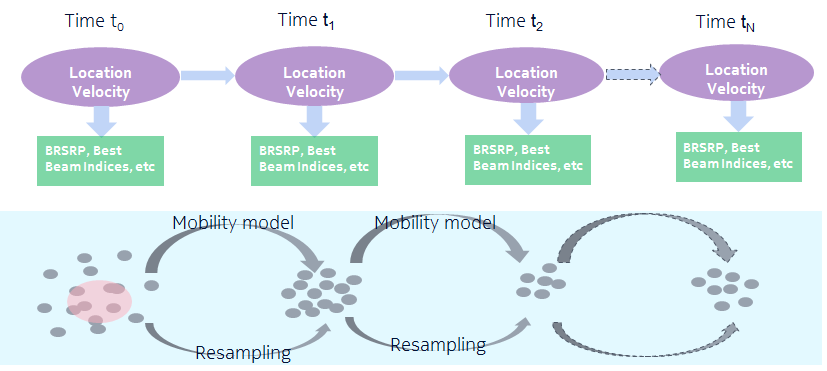
\includegraphics[height=3.5in,width=3.2in]{./HMM_ParticleFilter_Illustration.png}
	\caption{\label{fig:hmm_particle}
	{\small Hidden Markov Model and Particle filter}}
	\end{center}
	\end{figure}

\subsection{State transition probabilities and mobility model} 
\label{sec:statemodel}
These transition
probabilities model how transition happens from one hidden state
to another. 
We assume a suitable mobility model of the mobile which determines how it moves
along the graph $G_r$ and also helps us to calculate the above probabilities. We
assume that the mobile updates its speed according to Gauss-Markov Mobility Model ~\cite{Camp2002}.

\begin{align}
S_t = \alpha S_{t-1}+(1-\alpha)\bar{S}+\sqrt{(1-\alpha^2)}S_{x_{t-1}}
\label{eqn:speed}
\end{align}
\begin{align}
d_t = \alpha d_{t-1}+(1-\alpha)\bar{d}+\sqrt{(1-\alpha^2)}d_{x_{t-1}}
\label{eqn:speed}
\end{align}

 where $S_t$ and $d_t$ are the new speed and direction of the mobile at time interval t. $S_{t-1}$ and $d_{t-1}$
 are random variables from a Gaussian distribution with mean $\bar{S}$ and $\bar{d}$.
 
 At each time interval the next location is calculated based on the current location, speed, and direction of movement.
Specifically, at time interval t, a mobile's position is given by the equations.

\begin{align}
	x_t = x_{t-1} +S_{t-1}cos(d_{t-1})*\Delta t
\label{eqn:mobilitymodelx}
\end{align}
\begin{align}
y_t = y_{t-1} +S_{t-1}sin(d_{t-1})*\Delta t
\label{eqn:mobilitymodely}
\end{align}

where ($x_t$,$y_t$) and ($x_{t-1}$,$y_{t-1}$) are the x and y coordinates of the mobile’s position 
at the $t$th and ($t-1$) st time intervals, respectively. $\Delta t$ is the duration of the time interval.

\begin{algorithm}
\caption{$5GLocalizeAlgo(\mathcal{D}_{tr},G,N_{th})$}
\label{alg:LocalizeUEpf}
\begin{algorithmic}[1]
\State Offline inference based on training data $\mathcal{D}_{tr}$. This does not need real time processing.
\State Sample $N$ particles $\mathcal{P}_j = \{\hat{x}_1^{(j)},\hat{v}_1^{(j)}\},$ $j=1,\hdots , N$ 
from prior distribution $p(\tilde{x}_1, \tilde{v}_1|G)$ 

\State Initialize importance weights $\hat{w}_1^{(n)} \gets p(\{\tilde{R}^j_1\}_{j=1}^4,\{\tilde{B}^j_1\}_{j=1}^4|\hat{x}_1^{(n)}),$ $n=1,\hdots , N$

\State Normalize $w_1^{(n)} \gets \hat{w}_1^{(n)}/\sum_{l=1}^N \hat{w}_1^{(l)},$ $n=1,\hdots , N$

\For{$i = 2$ to $m$}
	\For{$n=1$ to $N$}
		\State Sample $\hat{x}_i^{(n)}$ from $\hat{x}_{i-1}^{(n)}$ based on state transition model in section ~\ref{sec:statemodel}.
		\State Update weight $\hat{w}_i^{(n)} \gets \hat{w}_{i-1}^{(n)} \times p(\{\tilde{R}^j_i\}_{j=1}^4, \{\tilde{B}^j_i\}_{j=1}^4|\hat{x}_{i}^{(n)})$ 
	\EndFor
	\State Normalize $w_i^{(n)} \gets \frac{\hat{w}_i^{(n)}}{\sum_{l=1}^N \hat{w}_i^{(l)}}$
	\State $\hat{N}_{eff} \gets \frac{1}{\sum_{l=1}^N (w_{i}^{(l)})^2}$
	\If{$\hat{N}_{eff} < N_{th}$, $i<m$, resampling condition satisfied}
		\State Sample $N$ particles with replacement from current particle set $\{\mathcal{P}_j\}_{j=1}^N$ with probabilities $\{\hat{w}_i^{(j)}\}_{j=1}^N.$ Update particle set with the new sampled set
		\State $w_i^{(n)} \gets \frac{1}{N}$ for $n=1,\hdots , N$
	\EndIf
\EndFor
\State $n^* = \arg \max_{n = 1 , \hdots, N} w_m^{(n)}$

\State Output location estimate $\{\hat{x}_i^{(n^*)}\}_{i=1}^m$ 
\State Output distribution \\
$p(\{\hat{x}^{(n)}\}_{i=1}^m|\{\tilde{R}^{1,2,3,4}_i\}_{i=1}^m,\{\tilde{B}^{1,2,3,4}_i\}_{i=1}^m,G) = w_m^{(j)}$ for $n=1$ to $N$
\end{algorithmic}
\end{algorithm}  
\section{Observation modeling using machine learning}
\label{sec:channel-model}
As mentioned in the above section, one of the important inference of HMM is the likelihood of observation metric at given state. In this section, we discuss how to infer the likehihood based 
on the observation metrics, i.e., SSSRP and beam indices in 5G network. 
\subsection{Inference on likelihood of beam indices}
\label{sec:prob-classification}
As part of the observations of HMM model, UE reports up to four observed best beam indices. The probability
distribution (also called the likelihood function) of a particular observed beam indices as its $j$-th ($j=1, 2, 3, 4$) best reported beam indices
at a given location is denoted by
$p(\tilde{B}^j_i|\hat{x}_{i})$. In our approach, these probabilities
can be learnt from the drive test data using machine learning classification algorithms.
There are different machine learning classifier in the literature. We use random forest classifier to segment the area into locations where the coverage of beam indices
exhibit strong spatial correlation. Note that during the study, we have tried different classifier and random forest indeed presents the best results.

The classification steps are as follows:

\begin{enumerate}

\item For each location, each base station that can be heard at that location, we
take the corresponding drive test data beam indices. 

\item For each cell, model the likelihood of a certain classification (beam indices) using {\em Random Forest} where the latitude and the longitude are 
taken as features of the model and the likelihood of the beam indices is the output. Each such {\em
Random Forest} is trained using data aggregated in previous step.

\item In this paper, we use the random forest classifier in the machine learning library (sklearn) to predict the probability of 
reporting a specific beam indices. The function $predict\_proba(X)$ can be used to get the probability of class $X$. 

\end{enumerate}
\subsection{Inference on likelihood of SSSRP}
\label{sec:prob-reg}
The SSSRP reported at different states
is part of the observations of HMM model. The probability
distribution (also called the likelihood function) of an observed SSSRP on a location is denoted by
$p(\tilde{R}_i|\hat{x}_{i})$. In our approach, these probabilities
can be learnt from the training data using machine learning regression algorithms. 
There are different machine learning regression algorithm in the literature.
However, SSSPR has the following two special properties:
\begin{itemize}
	\item The drive test data is spread over a non-contiguous location because coverage
	areas in a cell are not necessarily connected.
	\item  Wireless SSSRP manifests quite different properties in different locations
\end{itemize}

Thus, we use random forest regressor to segment the area into locations where the SSSPRs
exhibit strong spatial correlation. 

The regressions steps are as follows:

\begin{enumerate}
\item For each location, each base station and each reported beam indices that can be heard at that location, we
take the empirical mean and standard deviation of all corresponding drive test data
SSSRP. 

\item For each cell and each beam indices, model the spatial variation of SSSRP-statistics (i.e., mean and
standard deviation) using {\em Random Forest} where the latitude and the longitude are 
taken as features of the model and the SSSRP-statistic  of the cell is the output. Each such {\em
Random Forest} is trained using data aggregated in previous step. Also,
compute the mean square error (or {\em cross validation error})
for each random forest. 

\item Denote by $RndFrst_m(x,b,c)$ ($RndFrst_s(x,c)$) the random forest predictor of
mean (standard deviation) of SSSRP for cell-$c$, beam-$b$
at location $x$. Let $(\sigma_{RF}(b,c))^2$ be the corresponding
mean square error of the predictor. Then we model
\begin{align}
p(\tilde{R}^j_i|\hat{x}_{i}, \tilde{B}^j_i) =
\mathcal{N}(RndFrst(\hat{x}_{i},b,c), \sigma_c^2(\hat{x}_i))\ ,
\label{eqn:rndfrst}
\end{align}
where $$\sigma_c^2(x) = RndFrst_s(x,b,c) + \sigma_{RF}^2(b,c)\,$$ 
and the serving cell-$c$ can be obtained from the LUMD record. In general, we
can choose any spatial regressor instead of random forest. However, choosing
random forest makes the model robust to cell propogation properties and to the
fact that the coverage area of the cell could be disjoint.
\end{enumerate}

Note that in LTE network, the regression algorithm is implemented per cell. However, in 5G, with the existence of
beam indices, the regression algorithn is now implemented per cell and per beam indices.


\subsection{Inference on the likelihood of combined observations}
\label{sec:prob-combined}
The likelihood of seeing all the observations, $\{\tilde{R^j_i}\}_{j=1}^4$ and $\{\tilde{B^j_i}\}_{j=1}^4$ at a given location $\hat{x}){i}$ is as follows:

\begin{equation} 
\begin{split}
	p(\tilde{R}^1_i, \tilde{R}^2_i, \tilde{R}^3_i,\tilde{R}^4_i, \tilde{B}^1_i, \tilde{B}^2_i, \tilde{B}^3_i, \tilde{B}^4_i|\hat{x}_{i})
	\\
	=\prod_{j=1}^4 p(\tilde{R}^j_i|\hat{x}_{i}, \tilde{B}^j_i)p(\tilde{B}^j_i|\hat{x}_{i}),
\end{split}
\label{eqn:combined}
\end{equation}

%%%%%%%%%%%%%%%%%%%%%%%%%%%%%%%%%%%%%%%%%%%%%%%%%%%%%%%%%%%%%%%%%%%%%%%%%%%%%%%%%%%%%%%%%%
%\iffalse

\section{Extension: Joint Localization and Channel Modling}
\label{sec:extensionalgo}
In this section we describe our main algorithm for joint observation modeling and UE
localization. The Joint Observation Modeling and Localization (JOML) algorithm takes
as input the labeled and unlabeled datasets $\mathcal{D}_1,\mathcal{D}_2,$ the
graph $G$ and a parameter $N_{em}$ specifying the number of
expectation-maximization (EM) iterations to be performed. It outputs the UE
location estimates $\{\hat{x}_i\}_{i=1}^m$ and the observation model $\mathcal{C}$
in the region of interest. The main idea is to use expectation-maximization
procedure to iteratively improve the estimates of both the observation model
$\mathcal{C}$ and the location estimates $\{\hat{x}_i\}_{i=1}^m.$ The basic EM
algorithm improves the channel in each iteration from the previous according to
the following equation.

\begin{equation}
\mathcal{C}^{t+1} = \arg \max_{\mathcal{C}} E_{\{\hat{x}_i\}_{i=1}^m |\mathcal{D}_1,\mathcal{D}_2,\mathcal{C}^t} \log  P(\mathcal{D}_1,\mathcal{D}_2,\{\hat{x}_i\}_{i=1}^m|\mathcal{C}) \label{eq:EM}
\end{equation}

The high level pseudo-code of the algorithm is shown in Algorithm \ref{alg:joint_ch_model_loc}.  

%\begin{algorithm}
%\caption{$JCML(\mathcal{D}_1, \mathcal{D}_2, G, L_{th})$}
%\label{alg:joint_ch_model_loc}
%\begin{algorithmic}[1]
%\State $\mathcal{D} \gets \mathcal{D}_1$
%\State $\mathcal{C} \gets ChannelModel(\mathcal{D})$
%\For{$i=1$ to $m$}
%	\State $\{\hat{x}_j\}_{j=1}^i \gets %LocalizeUE(\{\tilde{R}_j,T_j\}_{j=1}^i,\mathcal{C},G)$ \label{step:localize}
%	\State $\mathcal{D} \gets \mathcal{D}_1 \cup %\{\tilde{R}_j,\hat{x}_j\}_{j=1}^i$
%	\State $\mathcal{C} \gets ChannelModel(\mathcal{D})$
%\EndFor
%\State Output $\{\hat{x}_i\}_{i=1}^m, \mathcal{C}$
%\end{algorithmic}
%\end{algorithm}  

\begin{algorithm}
\caption{$JOML(\mathcal{D}_1, \mathcal{D}_2, G, N_{em})$}
\label{alg:joint_ch_model_loc}
\begin{algorithmic}[1]
\State $\mathcal{C} \gets Observation Model(\mathcal{D}_1)$ based on section ~\ref{sec:channel-model}.
\For{$j = 1$ to $N_{em}$}
	\State $\{\hat{x}_i\}_{i=1}^m, p(\{\hat{x}_i,\tilde{R}^j_i,\tilde{B}^j_i\}_{i=1}^m|\mathcal{C},G) \gets 5GLocalizeUE(\mathcal{D}_2,\mathcal{C},G)$ as in Algorithm \ref{alg:LocalizeUEpf}. \label{step:localize}
	\State $\mathcal{D} \gets \mathcal{D}_1 \cup \{\tilde{R}_i,\hat{x}_i\}_{i=1}^m$ \label{line:em_approx}
	\State $\mathcal{C} \gets Observation Model(\mathcal{D})$ based on section ~\ref{sec:channel-model}.
\EndFor
\State Output $\{\hat{x}_i\}_{i=1}^m = \arg \max_{\{\hat{x}_i\}_{i=1}^m} p(\{\hat{x}_i,\tilde{R}_i, \tilde{R}_i\}_{i=1}^m,|\mathcal{C},G)$
\State Output $\mathcal{C}$
\end{algorithmic}
\end{algorithm}  

Note that in line \ref{line:em_approx} $\{\hat{x}_i\}_{i=1}^m$ can be the mode
or samples from the distribution
$p(\{\hat{x}_i,\tilde{R}^j_i, \tilde{B}^j_i\}_{i=1}^m,|\mathcal{C},G)$ as a stochastic
approximation for the EM algorithm. The JOML algorithm uses two main
subroutines. The first subroutine $ObservationModel$ computes the likelihood function
$\mathcal{C}$ from the labeled dataset $\mathcal{D}.$ $\mathcal{C}$ can be
viewed as a function which can output the distribution of SSSRP and beam indices from any base
station $k$ to any UE location $x \in V.$ The second subroutine $5GLocalizeUE$
use the observation model function $\mathcal{C},$ the LUMD data
$\{\tilde{R}_i,T_i\}$ and the graph $G$ to come up with location estimates of
the UE $\{\hat{x}_i\}_{i=1}^m$ and its corresponding distribution as illustrated in section ~\ref{sec:localalgo}. Each time a
location estimate is computed it is used with the corresponding record
$\tilde{R}^j_i$, $\tilde{B}^j_i$ and the dataset $\mathcal{D}_1$ to further improve the channel
model using an expectation-maximization procedure. Therefore in the next
iteration we can obtain a better location estimate. 

%\fi
%%%%%%%%%%%%%%%%%%%%%%%%%%%%%%%%%%%%%%%%%%%%%%%%%%%%%%%%%%%%%%%%%%%%%%%%%%%%%%%%%%%%

\section{Evaluation}
\label{sec:eval}

In this section, we present evaluation of our proposed technique. The objective of
our evaluation is three folds: to understand the accuracy of our localization scheme, to evaluate
how much the accuracy depends of fraction of network coverage area that is drive
tested.

\subsection{Methodology}
In this paper, we focus on one isolated cell in 5G network, which is the measurement report
only has the information of the serving cell. In the field, when we have multiple cells, the additional
information on the measruement report from neigboring cells can be easily incoorbated into the proposed algorithm and improve the 
localization accuary. As there is no commercial deployed 5G network yet, we dont have the drive test data from the field.
Instead, we use our 5G system simulator to generate both training data and test data.

The 5G system we use in this evaluation is operating at mmwave band, and the cell ISD is 100m. The testing data points are illustrated in 
Figure ~\ref{fig:training}. Instead of diving the training data into training and validation, we use the gridsearchCV and cross validation functionaility in 
sklearn ~\cite{sklearn} to avoid the overfitting since we have limited number of training data.

\begin{figure}[t]
	\begin{center}
	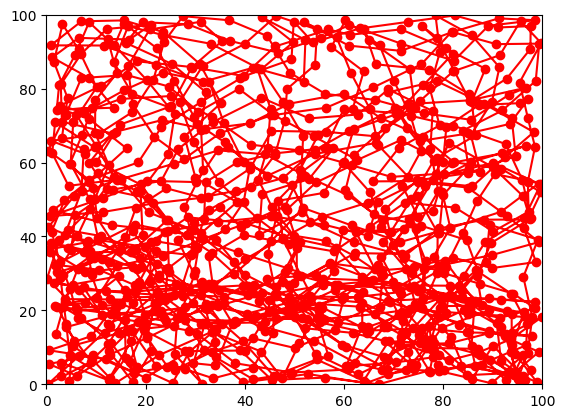
\includegraphics[height=2.4in,width=3.2in]{./GM_training.png}
	\caption{\label{fig:training}
	{\small Training data points}}
	\end{center}
	\end{figure}		

\subsection{Localization Results}


\begin{figure}[t]
\begin{center}
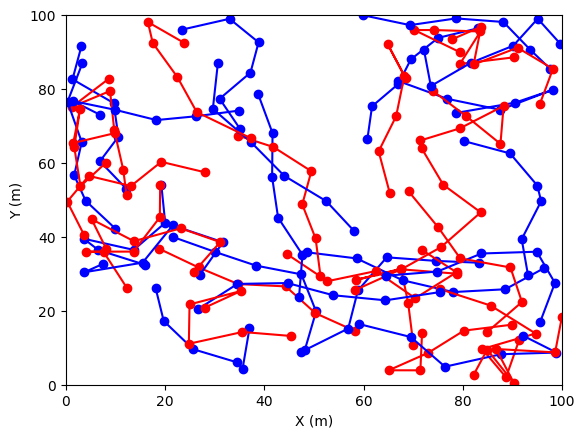
\includegraphics[height=2.4in,width=3.2in]{./Combined_path_illustration.png}
\caption{\label{fig:toyeg}
{\small Comparison of actual (red) and predicted (blue).}}
\end{center}
\end{figure}


In Figure ~\ref{fig:toyeg}, we show the predicted and actual locations of all mobiles. As it can be seen, the actual locations
and the estimated locations are quite close. In the following, we present more
detailed analysis of the results.

\begin{figure}[t]
	\begin{center}
	\subfigure[]{
	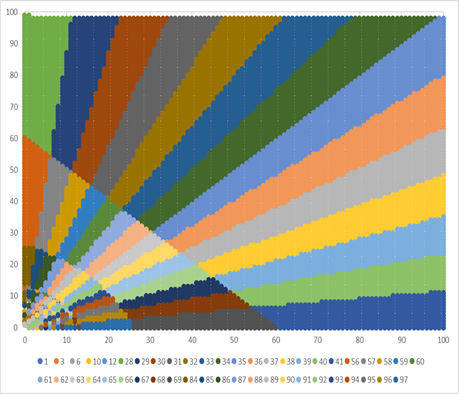
\includegraphics[height=2.5in, width=3.3in]{./Beam_map_LoS.png}
	%\caption{True Beam map for LoS}
	\label{fig:beam_map_cdf1}}
	\subfigure[]{
	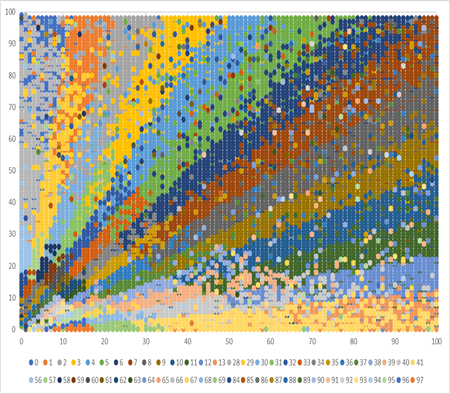
\includegraphics[height=2.5in, width=3.3in]{./Beam_map_MixedLoSNLoS.png}
	 %\caption{True Beam map for mixed LoS & NLoS}
	\label{fig:beam_map_cdf2}}
	\subfigure[]{
		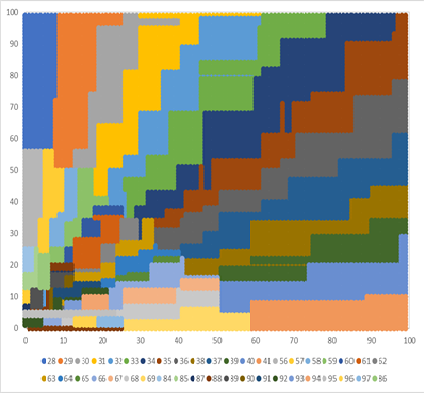
\includegraphics[height=2.5in, width=3.3in]{./Prediction_Beam_LoS.png}
	%	\caption{Predicted Beam map for LoS}
		\label{fig:beam_map_cdf3}}
		\subfigure[]{
	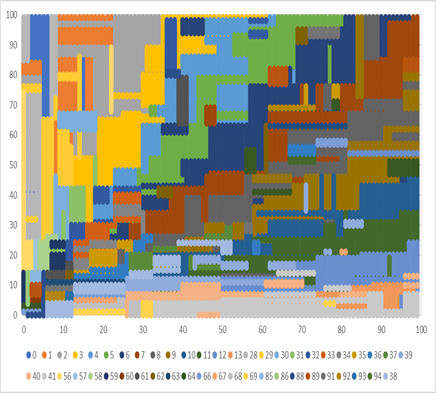
\includegraphics[height=2.5in, width=3.3in]{./Prediction_Beam_MixedLoSNLoS.png}
	%\caption{Predicted Beam map for NLoS}
	\label{fig:beam_map_cdf4}}
	\caption{Reported best beam indices distribution map \label{fig:leapperf} with different RF channel condition (LoS vs. MixedLoS\&NLoS)}
	\end{center}
	\end{figure}

\begin{figure}[t]
\begin{center}
\subfigure[]{
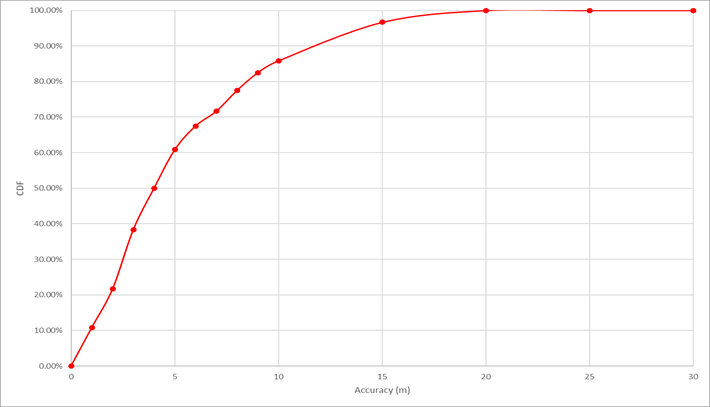
\includegraphics[height=2.5in, width=3.3in]{./Accuracy_cdf_LoS.png}
\label{fig:cdf1}}
\subfigure[]{
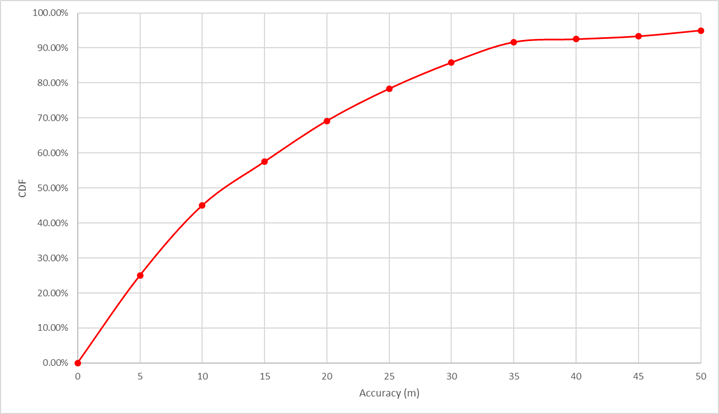
\includegraphics[height=2.5in, width=3.3in]{./Accuracy_cdf_MixedLoS_NLoS.png}
\label{fig:cdf2}}
\caption{CDF of accuracy.\label{fig:leapperf} with different RF channel condition (LoS vs. MixedLoS\&NLoS)}
\end{center}
\end{figure}
{\em Inference accuarcy} 
Figure~\ref{fig:beam_map_cdf1} and Figure~\ref{fig:beam_map_cdf2} illustrate the beam indices at different locations when RF channel conditons are LoS and mixed LoS\&NLoS, respectively. Figure~\ref{fig:beam_map_cdf3} and Figure~\ref{fig:beam_map_cdf4}
shows the predicted beam indices using random forest classification. As we can see from these figures, when the training data is more spreaded as shown in Figure ~\ref{fig:beam_map_cdf2},
the random forest classifier will divided the whole area into smaller region. The accuracy sore for LoS is 0.78 and for mixed LoS\&NLoS case is 0.57.

{\em Accuracy CDF:} In Figure~\ref{fig:cdf1} and Figure~\ref{fig:cdf2}, we show the
accuracy distribution under two different type of RF channel condition, line of sight (LoS) vs. Mixed LoS \& NLoS. The RF channel scenarios are illustrated in
~\cite{3gpp38901}. With LoS channel, the median accuracy is around
$4m$ and with Mixed LoS and NLoS channel, the median accuracy is around $12m$.These results have not included additional constraints such as that users move on prescribed paths such was walkways etc. as well as additional columns in the data matrix such as TA, etc. 
With the additional information, the localization accuracy is expected to improve further.

The rationale behind localizing the path taken by a mobile is two-fold: first,
localization accuracy of the individual points can be improved if there is a
nearby point that is more accurately localized; and second, we also make use the
road network to constrain points to lie on the road whenever the mobile is
moving. 



\section{Concluding Remarks}
\label{sec:concl}

% In this paper, we have developed localization algorithms of measurement records in
% LTE networks and we have also shown that measurement records can classified as indoor
% or outdoor with appropriate training. We have shown median accuracy of 20m in urban
% settings which is a significant improvement over more than 100m accuracy reported
% with non machine learning based techniques. A more challenging problem is to identify
% indoor locations at least in terms of buildings. This could require more training or
% combining LUMD with Wi-Fi signatures available from mobiles.




%{
%\bibliography{community_bibliography}
%\bibliographystyle{unsrt}    
%}          

{%\scriptsize
\bibliographystyle{acm}
\bibliography{myref}
}


\end{document}


